\documentclass[a4paper,10pt]{article}
\usepackage[utf8]{inputenc}
\usepackage{amsmath,mathrsfs}\usepackage{amsmath,amsfonts,amssymb,float,graphicx,mathtools,mathrsfs,tikz,amsthm}


\usepackage{standalone}
\usepackage{caption}
\usepackage{tikz}
\usetikzlibrary{positioning}
\usetikzlibrary{calc}
\usetikzlibrary{backgrounds}
\usepackage{tikzsymbols}
\usepackage{hieroglf}
\usepackage{nameref}
\usepackage{algpseudocode}
\usepackage{hyperref}
\usepackage{natbib}
\usepackage{booktabs}
\usepackage{stackengine}


\definecolor{tip}{rgb}{0.84,0.1,0.11}
\definecolor{branch}{rgb}{.48, .2, .58}
\definecolor{node}{rgb}{.17, .48, .71}
\definecolor{T}{rgb}{.65,.38,.1}

%opening
\title{MTBD models with partner notification}
\author{Anna Zhukova}

\begin{document}

\maketitle

%\begin{abstract}
%
%\end{abstract}

\section{Introduction}
The interaction of epidemiological and evolutionary processes leaves a footprint in pathogen genomes. Phylodynamics leverages this footprint to estimate epidemiological parameters~\citep{Grenfell2004a,Volz2013}. It relies on models that bridge the gap between traditional epidemiology and sequence data by estimating such parameters as the basic reproduction number, $R_0$, from topology and branch lengths of pathogen phylogenies (i.e. genealogies of the pathogen population, approximating the transmission trees) combined with metadata on the samples. This is particularly useful for emerging epidemics, when not enough data (e.g. incidence curves) might be gathered for accurate estimations with classic epidemiological methods, while using genetic data for phylodynamic estimations can provide valuable insights and help prevent epidemic spreads (e.g. accurate estimation of the infectious period is crucial for adjusting health policies for self-isolation).


Phylodynamic models can be classified into two main families:  coalescent~\citep{Volz2009a,Drummond2005,Pybus2000a} and birth-death (BD)~\citep{Kendall1948,Maddison2007,Stadler2009,Stadler2010}. Coalescent models are often preferred for estimating deterministic population dynamics, however for highly stochastic processes, such as the dynamics of emerging pathogens, BD models are better adapted~\citep{Macpherson2021}. In the classic BD model with incomplete sampling~\citep{Stadler2009}, births represent pathogen transmission events (happening at a constant transmission rate), while deaths correspond to becoming non-infectious (e.g. due to healing, self-isolation, starting a treatment, or death, modelled with a constant removal rate). 

The epidemic spread and detection can however be non-homogenous and depend on different factors, including governmental health policies (e.g. quarantine measures or development of pathogen detection tests), pathogen evolution over time (e.g. some SARS-CoV-2 variants are more transmissible than other),  differences between host individuals (e.g. due to their immune system particularities or to their behaviour).

To allow for heterogeneity at the population level, the multi-type birth-death (MTBD) extention of the classical BDS model was developed by~\citet{Stadler2013a}. MTBD framework allows for different types of individual states (and changes between them, modelled with state change rates). These models are phylodynamic analogies of compartmental models in classical epidemiology (e.g. SIR, Susceptible-Infectious-Removed).  Examples of the MTBD family models include the birth-death exposed-infectious (BDEI) model, which was designed for pathogens featuring an incubation period between the moments of infection and of becoming infectious (e.g. Ebola and SARS-CoV-2), and the birth-death with superspreading model (BDSS) accounting for the fact that some individuals might spread the pathogen more than the others~\citep{Stadler2014}.

To allow for heterogeneity over time, \citet{Stadler2013} developed one-state Bayesian birth-death skyline plot (BDSKY) that divides the time into intervals and allows for different piecewise constant rates on them. \citet{Kuhnert2016} combined the MTBD model with the BDSKY to allow for both piecewise-constant rate changes over time and multiple individual types. In particular the skyline approach can be useful to account for changes in the sampling policies (e.g. before/after HIV discovery or before/after PCR test spread for SARS-CoV-2).


Another important source of heterogeneity that none of these models accounts for is inflicted by non-random sampling. We can propose different sampling probabilities for different types of individuals in MTBD framework, or change of the sampling probability over time intervals with the BDSKY, however, none of them can account for non-randomness of sampling, in particular due to contact tracing and partner notification. 

In this study we propose an extension of the BD model that allows for modeling non-random sampling due to partner notification (PN), BD-PN. In the rest of the article, we describe the BD-PN model and its assumptions, present a transmission tree simulator under this model, derive the equations for BD-PN likelihood calculation, and propose a test for detecting partner notification in pathogen phylogenetic trees. We also present a maximum likelihood parameter estimator for BD-PN, and test it on simulated data. Finally, we apply it to the study of HIV-1 B epidemic in the UK. 


\section{BD-PN Framework}
In a pathogen transmission tree $\mathscr{T}$ (approximated by a time-scaled pathogen phylogeny) the tips represent sampled pathogens %, patient state transitions occur along the branches, 
while bifurcations (i.e. internal nodes) correspond to pathogen transmissions (Fig.~\ref{fig:tt}). The tree branches are measured in units of time, where $T$ is the time that passed between the tree root (the beginning of the (sub-)epidemic) and the last sampled tip. 


\begin{figure*}[tbhp]
\centering 
%\includegraphics[width=0.8\textwidth]{Transmission_tree.png}
\includestandalone[width=0.6\textwidth]{Fig_tree}
\caption{A transmission tree $\mathscr{T}$ with $n=5$ external nodes (i.e. tips, which correspond to sampling events: $0000, 0001, 001, 010, 011$), $n-1=4$ internal nodes (which correspond to transmissions: $0$ (the root) and $00, 01, 000$) and $2n - 2 = 8$ branches (plus the root branch of zero length). %The lengths of the branches are shown on the right of each branch: $t_i$ is the lengths of the branch connecting the node $i$ to its parent. 
Time $t$ starts at the root of the tree ($t=0$) and goes till the last sampled tip. The times of the nodes are shown on the left, e.g. $t_{0001}$ is the time of tip $0001$ (when $0001$'s pathogen was sampled). $T$ corresponds to the end of the sampling period (when the most recent tip, $0000$, was sampled).}
\label{fig:tt} 
\end{figure*}

\subsection{BD Model with incomplete sampling}
Under the basic birth-death model~\citep{Stadler2009} all the individuals are in the same state. They can transmit with a constant rate $\lambda$, get removed with a constant rate $\psi$, and their pathogen can be sampled upon removal with a constant probability $\rho$. 

%A general MTBD model describes $m$ possible individual states. An individual in state $k \in 1:m$ can be removed (i.e., become non-infectious, e.g., due to healing, starting a treatment, self-isolation, or death) at a rate $\psi_k$, change their state to a state $l \in 1:m$ at a rate $\mu_{kl}$ (where $\mu_{kk} = 0$), and transmit their pathogen to an individual in a state $l \in 1:m$ at rate $\lambda_{kl}$. Upon $i$'s removal, their pathogen can be sampled (and hence observed as a tip in the transmission tree) with a probability $\rho$. 

This model can be described with master equations representing the likelihood densities of evolving as on the observed transmission tree, with time $t$ going forward from the root ($t=0$) till the time of the last sampled tip ($t=T$). These likelihood densities depend on the probability $U(t)$ of an unobserved transmission tree that started from one individual at time $t$ and evolved till $T$, without them or any of their induced cases being sampled: 

\begin{equation}
\scriptsize
\begin{cases}
\dot{U}(t) = &\Big(\lambda + \psi\Big) U(t)\; \textit{\color{gray} $\leftarrow$ no event in the next infinitesimal time $\Delta t$ }\\
    &- \lambda U^2(t) \;  \textit{\color{gray} $\leftarrow$ transmission, followed by unsampled evolutions of both subtrees}\\
    &- \psi (1 - \rho)\;  \textit{\color{gray} $\leftarrow$ removal without sampling}\\
U(T) = & 1\;  \textit{\color{gray} $\leftarrow$ the probability to stay unsampled over time 0 is 1} \label{eq:Us}
\end{cases}
\end{equation}


With the equation~(\ref{eq:Us}), we can write down the equation for the probability density $p^{(i)}(t)$ of evolving as on an observed tree branch that finishes at time $t_i$, starting on this branch at a time $t \leq t_i$. The master equations for the BD models were initially developed by ~\citet{Stadler2009}, however what we present here, is their branch-specific formulation that we proposed in~\citep{zhukovaFastAccurateMaximumLikelihood2022}:

\begin{equation}
\scriptsize
\begin{cases}
\dot{p}^{(i)}(t) = & \Big(\lambda + \psi\Big) p^{(i)}(t)\; \textit{\color{gray} $\leftarrow$ no event in the next infinitesimal time $\Delta t$ }\\
    & - 2 \lambda p^{(i)}(t)U(t)\;  \textit{\color{gray} $\leftarrow$ transmission, where one of the subtrees stayed unsampled}\\
p^{(i)}(t_i) = 1
\end{cases}\label{eq:p}
\end{equation}

Using this equation, we can calculate the likelihood density $L(\mathscr{T}|\Theta)$ of a tree $\mathscr{T}$ under parameter values $\Theta = \{\lambda, \psi, \rho\}$ as:

\begin{equation}
\scriptsize
\begin{split}
log L(\mathscr{T}|\Theta) =  &\sum\limits_{i \in tips}  log(\psi \rho)  \textit{\color{gray} $\leftarrow$ sampling of $n$ tips} \\
 &+\sum\limits_{i \in \stackanchor{\tiny\textit{internal}}{\tiny\textit{nodes}}} log \big(2 \lambda p^{(i0)}(t_i)p^{(i1)}(t_i)\big)   \textit{\color{gray} $\leftarrow$ $n - 1$ transmission events,}\\
 & ~~~~~~~~~~~~~~~\textit{\color{gray} followed by child branch evolutions (each can be a donor)}  \label{eq:mtbd_tree_likelihood}
\end{split}
\end{equation}

The likelihood density can then be used to estimate model parameters from a phylogenetic tree (e.g. by finding parameter values that maximize it, in maximum likelihood framework). In particular, it permits inference of the following epidemiological parameters: 

\begin{itemize}
\item \textit{effective reproduction number} $R_e = \frac{\lambda}{\psi}$, expected number of individuals directly infected by an infectious case;
\item \textit{infectious time} $\frac{1}{\psi}$, time during which an infectious individual can further spread the epidemic.
\end{itemize} 

Importantly, the BD model is asymptotically unidentifiable (see Remark 3.4 in~\citep{Stadler2009}), but to become identifiable it requires one of the parameters to be fixed. In practice, it is often the sampling probability, as it may be approximated from epidemiological data $\rho$ (e.g., the proportion of sampled cases among the declared ones) or the infectious time $\frac{1}{\psi}$ (estimated from observations of infected cases). 


\subsection{PN extension}

We now propose a non-Markovian extension of the BD model that adds partner notification (PN).  In BD-PN, at the moment of sampling the sampled individual might notify their most recent partner with a given probability $\rho_n$. Upon notification, partner is removed almost instantaneously (modeled via a notified removal rate $\psi_p >> \psi$). BD-PN hence has 3 classical BD and 2 additional parameters:
\begin{itemize}
 \item $\lambda$ -- constant transmission rate: an infected individual transmits their pathogen to a newly infected individual (which corresponds to an internal node in the transmission tree);
 \item $\psi$ -- constant removal rate: an infected individual stops being infectious at this rate. This corresponds to a tip in the transmission tree (observed or hidden);
 \item $\rho$ -- constant sampling probability: upon removal the individual's pathogen might get sampled with this probability, which corresponds to an observed tip in the transmission tree;
 \item $\rho_n$ -- constant notification probability: upon sampling, the sampled individual might notify their most recent partner with this probability;
 \item $\psi_p >> \psi$ -- constant notified removal rate: a notified individual (if not yet removed via standard procedure) stops being infectious and gets observed with this rate. This creates an observed tip in the transmission tree.
\end{itemize}


This model is a simplification of the notification process, in particular it makes 4 assumptions:
\begin{enumerate}
\item only observed individuals can notify (instead of any removed individual);
\item notified individuals are always observed upon removal;
%\item notified individuals do not notify further;
\item after the notification, notified individuals do not transmit further;
\item only the most recent partner can get notified.
\end{enumerate}

These assumptions make the mathematics behind the model manageable, however they can be easily relaxed in a tree simulator (e.g., to be used with a deep learning estimator~\citep{Voznica2021}, which does not require likelihood calculation).

Note that the most recent partner relationship is not necessarily symmetrical, as the most recent partner of $i$ might have transmitted their virus further after the contact with $i$. 

\subsubsection{Mathematical formulation}
$p^{(i)}(t)$ in equations~(\ref{eq:p}) describes an evolution along a tree branch, provided that we do not know whether the individual at the end of the branch (at time $t_i$) is the same as at time $t$. These two individuals could be different if a hidden transmission, where the donor subtree stayed unobserved, occurred between times $t$ and $t_i$.

We will use an \textbf{oriented probability} $p^{(i,o)}(t)$ for the cases when the individual at the end of the branch is the same as at time $t$:

\begin{equation}
\scriptsize
\begin{cases}
\dot{p}^{(i,o)}(t) = & \Big(\lambda + \psi\Big) p^{(i,o)}(t)\; \textit{\color{gray} $\leftarrow$ no event in the next infinitesimal time $\Delta t$ }\\
    & - \lambda p^{(i,o)}(t)U(t)\;  \textit{\color{gray} $\leftarrow$ transmission, where the recipient subtree stayed unsampled}\\
p^{(i,o)}(t_i) = 1\label{eq:p-o}
\end{cases}
\end{equation}


Additionally we define a \textbf{non-hidden probability} $p^{(i,nh)}(t)$ for the cases when no hidden transmission occurred along the branch:

\begin{equation}
\scriptsize
\begin{cases}
\dot{p}^{(i,nh)}(t) = & \Big(\lambda + \psi\Big) p^{(i,nh)}(t)\; \textit{\color{gray} $\leftarrow$ no event in the next infinitesimal time $\Delta t$ }\\
p^{(i,nh)}(t_i) = 1\label{eq:p-nh}
\end{cases}
\end{equation}

The equations~\ref{eq:Us}, \ref{eq:p}, \ref{eq:p-o}, and \ref{eq:p-nh} have the following closed form solutions:
\begin{equation}
\scriptsize
\begin{split}
&\begin{cases}
U(t) = \frac{\lambda + \psi}{2\lambda} +  \frac{c_1}{2\lambda}\Big(\frac{E_1 - 1}{E_1 + 1}\Big)\\
\\
p^{(i)}(t) = \Big(\frac{E_2 + 1}{E_1 + 1}\Big)^2E_3 \\
\\
p^{(i,o)}(t) =  \frac{E_2 + 1}{E_1 + 1}\sqrt{E_3E_4} \\
\\
p^{(i,nh)}(t) =  E_4
\end{cases},\\
& \textit{where } c_1 = \sqrt{(\lambda - \psi)^2 + 4 \lambda\psi\rho},\; c_2 = \frac{c_1 + \lambda - \psi}{c_1 - \lambda + \psi},\\
& ~~~~~~~~E_1 = c_2 e^{c_1 (t -T)},\; E_2 = c_2 e^{c_1 (t_i -T)},\; E_3 = e^{c_1 (t -t_i)}, \; E_4 =  e^{(\lambda + \psi) (t -t_i)}\\
\end{split}\label{eq:ps}
\end{equation}


%Under the BD-PN model, the probability density $q(i)$ of a branch connecting a node $i$ to its parent node $j$ (without taking into account the event at the end of the branch) can be written as:
%
%
%\begin{equation}
%\scriptsize
%q(i) = 
%\begin{cases}
%q^{(u)}(i) = p^{(i)}(t_j) \textit{\color{gray} ~if $i$ is an \textbf{unnotified non-notifier}}\\
%q^{(n)}(i) = 
%p^{(i,nh)}(t_j) \textit{\color{gray} ~~if $i$ is a tip corresponding to a \textbf{notifier}}\\
%~~~~~~~~~~~~ \textit{\color{gray}(parent is the last transmission, no hidden transmission along the branch)}
%\\
%q^{(p)}(i)  = p^{(i, o)}(t_j)  \textit{\color{gray} ~if $i$ is an internal or tip node whose individual will be notified after $t_i$}
%\\
%q^{(p)}(i, r)  = p^{(r, o)}(t_j) e^{- \psi_p (t_i - t_r)} \textit{\color{gray} if $i$ is a \textbf{partner} tip notified by $r$ at time $t_r \leq t_i$}
%\end{cases}
%\label{eq:branch}
%\end{equation}

Using the formulas~(\ref{eq:ps}), we can calculate the likelihood density of a tree using a pruning algorithm~\citep{10.1093/sysbio/22.3.240}, where for each visited node $i$ we calculate the likelihood density of its subtree if the branch connecting it to its parent node $j$ corresponds to (1) an unnotified individual $l^{(u)}(i)$; or (2) an (eventually) notified partner $l^{(p)}(i, r)$ (notified by the individual corresponding to the tip $r$ at time $t_r$). For each visited tip we additionally consider whether the corresponding individual notified their most recent partner or not.

%For a tip $i$ in state $si$ these values can be calculated as:
%\begin{equation}
%\scriptsize
%\begin{array}{ll}
%l^{(u)}(i) &= \begin{cases} l^{(u,n)}(i) = q^{(u)}(i)\psi\rho
%\rho_{n} \textit{\color{gray} ~~~~~~~~if $i$ notified their most recent patner}\\
%l^{(u,\not{n})}(i) = q^{(u)}(i)\psi\rho (1-\rho_{n}) \textit{\color{gray} ~if $i$ did not notify}
%\end{cases}\\
%l^{(p)}(i, r) &= q^{(p)}(i,r)\psi_p\cdot \begin{cases}
%\rho_{n} \textit{\color{gray} ~~~~~~~~if $i$ notified their most recent patner}\\
%(1-\rho_{n}) \textit{\color{gray} ~if $i$ did not notify}
%\end{cases}\\
%\end{array}
%\label{eq:tip}
%\end{equation}


For a tip $i$ with a parent node $j$ these values can be calculated as:
\begin{equation}
\scriptsize
\begin{array}{ll}
l^{(u,n)}(i) &= p^{(i,nh)}(t_j)\psi\rho
\rho_{n} \textit{\color{gray} ~if $i$ was not notified but notified their most recent patner}\\
l^{(u,\not{n})}(i) &= p^{i}(t_j)\psi\rho (1-\rho_{n}) \textit{\color{gray} ~if $i$ was not notified and did not notify}\\
l^{(p,n)}(i,r) &= \begin{cases}
p^{(i, nh)}(t_j)\psi\rho\rho_{n} \textit{\color{gray} ~if $i$ got notified at time $t_r > t_i$ and notified their most recent patner}\\
p^{(r, nh)}(t_j) e^{- \psi_p (t_i - t_r)} \psi_p \rho_{n} \textit{\color{gray} ~if $i$ got notified at time $t_r \leq t_i$ and notified}
\end{cases}\\
l^{(p,\not{n})}(i,r) &= \begin{cases}
p^{(i, o)}(t_j)\psi\rho(1 - \rho_{n}) \textit{\color{gray} ~if $i$ got notified at time $t_r > t_i$ and did not notify}\\
p^{(r, o)}(t_j) e^{- \psi_p (t_i - t_r)} \psi_p (1-\rho_{n}) \textit{\color{gray} ~if $i$ got notified at time $t_r \leq t_i$ and did not notify}
\end{cases}\\
\end{array}
\label{eq:tip}
\end{equation}

Let us now consider an internal node $i$ with two child nodes, $i_0$ and $i_1$. We will start with the configuration where the $i$'s branch corresponds to an unnotified individual. We will consider three possibilities: (i) when both $i_0$ and $i_1$ are internal nodes; (ii) when both $i_0$ and $i_1$ are tips; and (iii) when one of them is an internal node and the other one is a tip.

%Note that a notification will only be possible if the notifying branch is external as the notifier only notifies the most recent partner, i.e. the transmission corresponds to the notifier's parent node.

First, let's assume that (i) $i_0$ and $i_1$ are internal. Then none of them can be a notifier (since notifiers correspond to tips), and hence none of them is notified:

\begin{equation}
\scriptsize
l^{(u)}(i) = p^{i}(t_j) 2\lambda l^{(u)}(i_0)l^{(u)}(i_1) \label{eq:lu-int-int}
\end{equation}

Secondly, let's assume that (ii) $i_0$ and $i_1$ are tips. Then each of them could have notified the other one:

\begin{equation}
\scriptsize
\begin{split}
l^{(u)}(i) = p^{i}(t_j) 2\lambda \cdot 
\Big(&l^{(u,\not{n})}(i_0)l^{(u,\not{n})}(i_1) \textit{\color{gray}~$\leftarrow$ neigher $i_0$ nor $i_1$ notified} \\
&+ l^{(u,n)}(i_0)l^{(p,\not{n})}(i_1,i_0) \textit{\color{gray}~$\leftarrow$ $i_0$ notified $i_1$ and $i_1$ did not notify} \\
&+ l^{(u,n)}(i_1)l^{(p,\not{n})}(i_0,i_1) \textit{\color{gray}~$\leftarrow$ $i_1$ notified $i_0$ and $i_0$ did not notify} \\
&+ l^{(p,n)}(i_0,i1)l^{(p,n)}(i_1,i_0)\Big) \textit{\color{gray}~$\leftarrow$ $i_1$ and $i_0$ notified each other} \\
\end{split}\label{eq:lu-tip-tip}
\end{equation}

Lastly, let's assume that (iii) $i_0$ is a tip and $i_1$ is internal (the scenario where $i_1$ is a tip and $i_0$ is internal can be obtained by swapping the labels). Then $i_0$ could have notified $i_1$:


\begin{equation}
\scriptsize
\begin{split}
l^{(u)}(i) = p^{i}(t_j) 2\lambda \cdot 
\Big(&l^{(u,\not{n})}(i_0)l^{(u)}(i_1) \textit{\color{gray}~$\leftarrow$ $i_0$ did not notify $i_1$ } \\
&+ l^{(u,n)}(i_0)l^{(p)}(i_1,i_0)\Big) \textit{\color{gray}~$\leftarrow$ $i_0$ notified $i_1$} \\
\end{split}\label{eq:lu-int-tip}
\end{equation}


%\begin{equation}
%\scriptsize
%l^{(u)}(i) = p^{i}(t_j) 2\lambda \\
%\cdot \begin{cases}
%l^{(u)}(i_0)l^{(u)}(i_1) \textit{\color{gray} ~if both $i_0$ and $i_1$ are internal} \\
%l^{(u,\not{n})}(i_0)l^{(u)}(i_1) + l^{(u,n)}(i_0)l^{(p)}(i_1,i_0) \textit{\color{gray}~if $i_0$ is a tip and $i_1$ is internal} \\
%l^{(u,\not{n})}(i_1)l^{(u)}(i_0) + l^{(u,n)}(i_1)l^{(p)}(i_0,i_1) \textit{\color{gray}~if $i_1$ is a tip and $i_0$ is internal} \\
%l^{(u,\not{n})}(i_0)l^{(u,\not{n})}(i_1) \\
%~~~~+ l^{(u,n)}(i_0)l^{(p,\not{n})}(i_1,i_0) + l^{(u,n)}(i_1)l^{(p,\not{n})}(i_0,i_1)\\
%~~~~+ l^{(p,n)}(i_0,i1)l^{(p,n)}(i_1,i_0) \textit{\color{gray}~if both $i_0$ and $i_1$ are tips} \\
%\end{cases}
%%& + is\_tip(i_0)l^{(u,n)}(i_0)l^{(p)}(i_1,i_0)\textit{\color{gray} $\leftarrow$ notification of someone in $i_1$'s subtree by $i_0$} \\
%%&+ is\_tip(i_1)l^{(u,n)}(i_1)l^{(p)}(i_0,i_1)~\Big) \textit{\color{gray} $\leftarrow$ notification of someone in $i_0$'s subtree by $i_1$},\\
%%\textit{where } & is\_tip(r) = 1 \textit{ if r is a tip and $= 0$ if r is an internal node.}\label{eq:lu}
%\end{equation}


In the other case an internal node $i$ corresponds to a partner who will eventually get notified by a node $r$. In this case the individual on the path connecting this branch to the notified tip stays the same (the partner). Hence, all the transmissions on this path are oriented and correspond to the partner transmitting to another recipient individual. %Moreover, this recipient's branch cannot be notified by our partner (as in our model notified partners do not notify further):
Again, we will consider three possibilities for $i$'s child nodes: (i) when both $i_0$ and $i_1$ are internal nodes; (ii) when both $i_0$ and $i_1$ are tips; and (iii) when one of them is an internal node and the other one is a tip.

In any of these scenarios, the notification must have happened after the partner tip branch start (as one of the model assumptions is that partners do not transmit after notification). Hence:
\begin{equation}
\scriptsize
l^{(p)}(i, r) = 0 \textit{~if $i$ is internal and $t_i > t_r$ or $i$ is a tip and $t_{parent(i)} > t_r$} \\
\label{eq:lp-zero}
\end{equation}

First, let's assume that (i) $i_0$ and $i_1$ are internal. Then none of them can be a notifier (since notifiers correspond to tips), and hence exactly one of them is notified (by $r$):

\begin{equation}
\scriptsize
\begin{split}
l^{(p)}(i, r) = p^{(i,o)}(t_j) \lambda \cdot
\Big(&l^{(p)}(i_0,r)l^{(u)}(i_1) \textit{\color{gray}~$\leftarrow$ $i_0$ is notified by $r$} \\
& + l^{(p)}(i_1,r)l^{(u)}(i_0)\Big) \textit{\color{gray}~$\leftarrow$ $i_1$ is notified by $r$} \\
 \end{split}
\label{eq:lp-int-int}
\end{equation}

Secondly, let's assume that (ii) $i_0$ and $i_1$ are tips. Then each of them could have notified the other one (in addition to one of them being notified by $r$):

 
\begin{equation}
\scriptsize
\begin{split}
l^{(p)}(i, r) = p^{(i,o)}(t_j) \lambda \cdot
\Big(&l^{(p,\not{n})}(i_0,first(r,i_1))l^{(u,n)}(i_1) \textit{\color{gray}~$\leftarrow$ $i_0$ got notified by both $r$ and $i_1$, but did not notify $i_1$} \\
&+ l^{(p,n)}(i_0,first(r,i_1))l^{(p,n)}(i_1, i_0) \textit{\color{gray}~$\leftarrow$ $i_0$ got notified by both $r$ and $i_1$, and notified $i_1$} \\
&+l^{(p,\not{n})}(i_1,first(r,i_0))l^{(u,n)}(i_0) \textit{\color{gray}~$\leftarrow$ $i_1$ got notified by both $r$ and $i_0$, but did not notify $i_0$} \\
&+ l^{(p,n)}(i_1,first(r,i_0))l^{(p,n)}(i_0, i_1) \textit{\color{gray}~$\leftarrow$ $i_1$ got notified by both $r$ and $i_0$, and notified $i_0$} \\
&+l^{(p,n)}(i_0,r)l^{(p,\not{n})}(i_1, i_0) \textit{\color{gray}~$\leftarrow$ $i_0$ got notified by $r$, and notified $i_1$} \\
& + l^{(p,n)}(i_1,r)l^{(p,\not{n})}(i_0, i_1) \textit{\color{gray}~$\leftarrow$ $i_1$ got notified by $r$, and notified $i_0$} \\
&+l^{(p,\not{n})}(i_0,r)l^{(u,\not{n})}(i_1) \textit{\color{gray}~$\leftarrow$ $i_0$ got notified by $r$, and did not notify $i_1$} \\
& + l^{(p,\not{n})}(i_1,r)l^{(u,\not{n})}(i_0)\Big) \textit{\color{gray}~$\leftarrow$ $i_1$ got notified by $r$, and did not notify $i_0$} \\
\textit{\color{gray}~where } &\color{gray}first(a,b) = 
\begin{cases}
a \textit{~if $t_a \leq t_b$}\\
b \textit{~if $t_a > t_b$.}
\end{cases} 
 \end{split}
\label{eq:lu-tip-tip}
\end{equation}

Lastly, let's assume that (iii) $i_0$ is a tip and $i_1$ is internal (the scenario where $i_1$ is a tip and $i_0$ is internal can be obtained by swapping the labels). Then $i_0$ could have notified $i_1$ (in addition to one of them being notified by $r$):


\begin{equation}
\scriptsize
\begin{split}
l^{(p)}(i, r) = p^{(i,o)}(t_j) \lambda \cdot
\Big(&l^{(p,n)}(i_0,r)l^{(p)}(i_1,i_0) \textit{\color{gray}~$\leftarrow$ $i_0$ got notified by $r$, and notified $i_1$} \\
& + l^{(p,\not{n})}(i_0,r)l^{(u)}(i_1) \textit{\color{gray}~$\leftarrow$ $i_0$ got notified by $r$, and did not notify $i_1$} \\
& +l^{(p)}(i_1,first(r,i_0))l^{(u, n)}(i_0) \textit{\color{gray}~$\leftarrow$ $i_0$ got notified by both $r$ and $i_0$} \\
& + l^{(p)}(i_1,r)l^{(u, \not{n})}(i_0)\Big) \textit{\color{gray}~$\leftarrow$ $i_0$ got notified by $r$} \\
\textit{\color{gray}~where } &\color{gray}first(a,b) = 
\begin{cases}
a \textit{~if $t_a \leq t_b$}\\
b \textit{~if $t_a > t_b$.}
\end{cases} 
 \end{split}
\label{eq:lp-tip-int}
\end{equation}


%\begin{equation}
%\scriptsize
%l^{(p)}(i, r) = p^{(i,o)}(t_j) \lambda
%\begin{cases}
%l^{(p)}(i_0,r)l^{(u)}(i_1) + l^{(p)}(i_1,r)l^{(u)}(i_0) \textit{\color{gray} ~if both $i_0$ and $i_1$ are internal} \\
%l^{(p,n)}(i_0,r)l^{(p)}(i_1,i_0) + l^{(p,\not{n})}(i_0,r)l^{(u)}(i_1) \\
%~~~~~~+ \begin{cases}
%l^{(p)}(i_1,first(r,i_0))l^{(u, n)}(i_0) \textit{\color{gray} ~if $t_{i0} \geq t_{i1}$}  \\
%0 \textit{\color{gray} ~if $t_{i0} < t_{i1}$}
% \end{cases}\\
%~~~~~~+ l^{(p)}(i_1,r)l^{(u, \not{n})}(i_0) \textit{\color{gray} ~if $i_0$ is a tip and $i_1$ is internal} \\
%l^{(p,n)}(i_1,r)l^{(p)}(i_0,i_1) + l^{(p,\not{n})}(i_1,r)l^{(u)}(i_0) \\
%~~~~~~+ \begin{cases}
%l^{(p)}(i_0,first(r,i_1))l^{(u, n)}(i_1) \textit{\color{gray} ~if $t_{i1} \geq t_{i0}$}  \\
%0 \textit{\color{gray} ~if $t_{i1} < t_{i0}$}
% \end{cases}\\
%~~~~~~+ l^{(p)}(i_0,r)l^{(u), \not{n}}(i_1) \textit{\color{gray} ~if $i_1$ is a tip and $i_0$ is internal} \\
%l^{(p,\not{n})}(i_0,first(r,i_1))l^{(u,n)}(i_1) + l^{(p,n)}(i_0,first(r,i_1))l^{(p,n)}(i_1, i_0)\\ 
%~~~~~~+l^{(p,\not{n})}(i_1,first(r,i_0))l^{(u,n)}(i_0) + l^{(p,n)}(i_1,first(r,i_0))l^{(p,n)}(i_0, i_1)\\
%~~~~~~+l^{(p,n)}(i_0,r)l^{(p,\not{n})}(i_1, i_0) + l^{(p,n)}(i_1,r)l^{(p,\not{n})}(i_0, i_1)\\ 
%~~~~~~+l^{(p,\not{n})}(i_0,r)l^{(u,\not{n})}(i_1) + l^{(p,\not{n})}(i_1,r)l^{(u,\not{n})}(i_0)
%\textit{\color{gray} ~if both $i_0$ and $i_1$ are tips} \\
% \end{cases}
%\label{eq:lu}
%\end{equation}

Note that $l^{(p)}(a, b)$ depends on the notifier $b$ and can only be calculated once the notification time is known, i.e. once we have climbed to an internal node corresponding to the transmission between the notifier (corresponding to one of its children, must be a tip) and the partner (the other child). The calculation is done recursively by descending into the subtree. However, as all the unotified equation parts ($l^{(u)}(i)$) only depend on the corresponding node $i$, they can be pre-calculated and reused to speed up the recursive steps.


%In the partner subtree only the contribution coming from the partner tip branch depends on the notification time. Hence while climbing the tree from tips to the root, for each internal node $i$ we can store an array of pre-calculated values for notified internal paths leading to each of its tips. The values of this array will store for each tip (e.g. $a$) its sampling time $t_a$ and a configuration $C(i,a)$, representing the subtree likelihood provided $a$ corresponds to the same notified partner individual as $i$ (but without the $a$'s tip branch contribution): 
%
%\begin{equation}
%\scriptsize
%\begin{split}
%C_{sj}(i,a) = &\begin{cases}
%1 \textit{\color{gray}~~~if $i = a$}
%\\
%q^{(p)}_{sj}(i)
%\sum\limits_{k=1}^{m}\lambda{si,k} \cdot l_{k}^{(u)}\Big(child(i, \not a)\Big)C_{si}\Big(child(i, a),a\Big) \textit{\color{gray}~~otherwise}\\ 
%\end{cases},
%\\ &\textit{where child(i,a) is the child of i whose subtree contains a},
%\\
% &\textit{~~~~~~~~child(i,$\not a$) is the child of i whose subtree does not contain a.}
%\end{split}
%\label{eq:c}
%\end{equation}

%Note that the path connecting $j$ to the parent of $i$ in this configuration corresponds to the same partner individual, hence this individual is the donor at all transmissions (internal nodes) on this path, hence at the moments of these transmissions the individual's state is known (as we only consider trees with known node states). At each internal node in this path the other branch (leading to a non-$j$'s subtree) corresponds to a recipient of the transmission occurring at that node, where the donor is the partner individual corresponding to $j$ (and $i$) and hence will not notify the recipient (as in our model's assumptions notified partners do not notify further).

%Once a potential notifier tip $r$ is identified (i.e., $r$ is a sister tip of the currently visited node $i$), we can calculate $l^{(p)}_{sj}(i, r)$ as:
%\begin{equation}
%\scriptsize 
%l^{(p)}_{sj}(i, r) = \sum\limits_{a \in tips(i)}C_{sj}(i, a) l^{(p)}_{sa}(a, r)\label{eq:lp}
%\end{equation}

\bigskip

The tree $\mathscr{T}$ likelihood density $\mathscr{L}(\mathscr{T}|\Theta)$ under BD-PN model with parameters $\Theta=\{\lambda, \psi, \rho, \psi_p, \rho_n\}$ can be calculated as $l^{(u)}(root)$, as the root can only correspond to an unnotified individual (since there was no observed transmission before it).

%The computational of $\mathscr{L}(\mathscr{T}|\Theta)$ includes $O(N^2)$ resolutions of system~(\ref{eq:p}) (for different times and initial conditions) in the worst case (caterpillar tree) and $O(NlogN)$ in the best case (for a balanced tree), where $N$ is the number of tips in $\mathscr{T}$.


\subsection{Extension to forests}

As we previously described in~\citep{zhukovaFastAccurateMaximumLikelihood2022}, the likelihood calculation with MTBD models can be easily extended to forests. This extension applies also to the BD-PN model. Forests are useful for cases when a (sub-)epidemic started with several infected individuals (e.g. due to multiple pathogen introductions to a country of interest or due to a change of health policies leading to a change in parameter values).

In this case the (sub-)epidemic leads to a forest $\mathscr{F}$ of $f$ observed trees: $\mathscr{T}_1, \ldots, \mathscr{T}_f$. The forest $\mathscr{F}$ might also include a certain number $u$ of unobserved trees, for which none of their tips got sampled.
Forest likelihood formula hence combines the likelihoods of $f$ observed and $u$ hidden trees, and can be represented in logarithmic form~(\ref{eq:forest_likelihood}). Tree likelihood formula %[\ref{eq:tree_likelihood}] 
is its special case, where $f=1$ and $u=0$. 

%As our application to Ebola data (see~Application) shows, $u$ is an important parameter: while the results are not very sensible to slight $u$ variations, ignoring it completely (e.g. using $u=0$ instead of $u \approx 500$ in our example) can change the inferences.

\begin{equation}
\begin{split}
logL(\mathscr{F}|\Theta,u)&=u\,logU_{hidden}(\Theta) + \sum\limits_{j=1}^f logL(\mathscr{T}_j|\Theta), \\
\textit{ where }& U_{hidden}(\Theta)=\sum\limits_{s=1}^{d}\pi_s U_s(t_{start}),\\
\textit{ and }& t_{start} \textit{ is the (potentially averaged) start time of the hidden trees.}
\end{split} \label{eq:forest_likelihood} 
\end{equation}

For given model parameter values $\Theta$ we can estimate the number of hidden trees $u$ from the number of observed trees $f$ as:
\begin{equation}
u = f \frac{U_{hidden}(\Theta)}{1 - U_{hidden}(\Theta)}\label{eq:u} 
\end{equation}



\section{Tree simulator}
We implemented a quick tree simulator that generates sampled transmission trees under MTBD and MTBD-PN models (with $m$ states). The simulator is Gillespie-based, generates state change, transmission and removal times, and only reconstructs the sampled parts of the tree to save memory and increase speed. 

The simulator iterates through occurring events till either time or sampled tip number limit is reached. 
It keeps updating an array $C = [c_1, \ldots, c_m]$ of counts of currently infected individuals (i.e. non-removed) in different states; an array $S = [s_1, \ldots, s_m]$ of counts of sampled individuals in different states; as well as a mapping $M$ between states and ids of currently infected individuals in those states, and a mapping $N$ between states and ids of sampled individuals in those states.  In the beginning ($t=0$) the only infected individual corresponds to the root: $c_k = 0 \;\forall k \neq state(root), \;c_{state(root)} = 1; \;M_k = \emptyset \; \forall k \neq state(root)$, $ \; M_{state(root)} = \{root\}$, and no individual is sampled: $s_k=0,\;N_k = \emptyset \; \forall 1 \leq k \leq m$.

At each iteration the algorithm (1) calculates the time of the next event; (2) chooses the type of this event and the the individual involved in it; (3) updates the counts and the mappings according to the event and records its time.

At step 1, to calculate the time of the next event, we (i) calculate the total rate $r$ as a sum of total state change, transmission and transition rates: $r = r^{(\mu)} + r^{(\lambda)} + r^{(\psi)}$, where $r^{(\mu)} = \sum\limits_{k=1}^{m} c_k \sum\limits_{r=1}^{m} \mu_{kr}$, $r^{(\lambda)} = \sum\limits_{k=1}^{m} c_k \sum\limits_{r=1}^{m} \lambda_{kr}$, and $r^{(\psi)} = \sum\limits_{k=1}^{m} c_k \psi_{k}$; (ii) draw $\Delta t$ from the exponential distribution with rate $r$; (iii) update the current time to $t + \Delta t$.

At step 2, to chose the type of the event, we draw a value $v$ (uniformly) from an interval $[0, r[$. This interval can be seen as composed of subintervals corresponding to each possible event, where the width of each subinterval is defined by the corresponding rate and infected individual count, e.g. the subinterval corresponding to a transmission from $k$ to $r$ has a width of $\lambda_{kr}c_k$. The subinterval in which $v$ is located defines the event type.

At step 3, we randomly draw an individual $i$ of type $k$ (selected at step 2) from $M[k]$, and proceed depending on the event type. If it is a state-change from $k$ to $r$, then we decrease $c_k$ by one, increase $c_r$ by one, remove $i$ from $M[k]$ and put $i$ into $M[r]$. If it is a transmission from $k$ to $r$, then we increase $c_r$ by one, create a new id $j$ for the recipient and put $j$ into $M[r]$. If it is a removal, then we decrease $c_k$ by one, remove $i$ from $M[k]$, and draw a value $p$ (uniformly) from an interval $[0, 1[$: if $p < \rho$, the individual gets sampled and we put $i$ into $N[k]$. 

For transmission and sampling events we also record their time and ids of the involved individuals. These values are used to reconstruct the sampled parts of the tree once the simulation is finished.


For the PN version of this simulator, we add an additional $m+1^{th}$ state for notified partners. $m + 1$'s state-change and transmission rates are set to zero: $\mu_{k,m+1} = \mu_{m+1,k} = \lambda_{k,m+1} = \lambda_{m+1,k} = 0\; \forall 1 \leq k \leq m$, while its removal rate is set to the notification removal rate: $\psi_{m+1} = \psi_p >> \psi_k\; \forall 1 \leq k \leq m$. We keep a mapping of most recent partners $P$ for each infectious individual, and update it for both the donor and the recipient at each transmission event. We also keep a mapping between each infectious individual and their state, and update it at each state-change event. At each removal event, we check whether the individual $i$ is a notified partner (i.e. in state $m+1$). If yes, we put them into $N[m+1]$ without performing the sampling probability draw. If not, and if $i$ gets sampled upon removal, we draw a value $p$ (uniformly) from an interval $[0, 1[$. If $p < \rho_n$, and if $i$'s most recent partner ($j = P[i]$) is not yet sampled (not in $N[state(j)]$), we change $j$'s state to $m + 1$ as in a state-change event.


\subsection*{Code availability}
The simulator is implemented in Python 3. It uses ETE 3 framework for tree manipulation~\citep{Huerta-Cepas2016} and NumPy package for array operations~\citep{harris_array_2020}. 

It is available as a command-line program and a Python 3 package via PyPi (\href{https://pypi.org/project/treesimulator}{treesimulator}), and via Docker/Singularity (\href{https://hub.docker.com/r/evolbioinfo/treesimulator/tags}{evolbioinfo/treesimulator}). Its source code and the installation and usage documentation are available on GitHub at \href{https://github.com/evolbioinfo/treesimulator}{github.com/evolbioinfo/treesimulator}.


\section{PN test}
To access whether a give tree is generated under a classical MTBD model or MTBD-PN, we developed a non-parametric test based on cherries (two tips having a common parent). 
The intuition behind the test is that in the presence of partner notification the tree will contain more cherries whose tips are close in time. 

The test sorts the cherries by the times of their roots, and splits them into blocks of 100 cherries (adjustable parameter). For each cherry in a block, the test calculates the difference between its tip times, hence obtaining an array of 100 cherry tip differences. It then generates a collection of random cherry tip differences for the same block: For each original cherry root it picks 5 more cherries with the roots that are the closest in time, randomly selects two tips among their tips, and calculates their time difference. An array of 100 reshuffled cherry tip differences is thus obtained fro the same block. The reshuffled cherry tip difference array generation is repeated 100 times (adjustable parameter). Finally, the test reports the proportion of reshuffled arrays whose first quantile is smaller than that of the real cherry array. 

The test therefore reports a probability of partner notification being present at time interval corresponding to each block. To estimate the probability of partner notification being present in the whole tree, it averages the block probabilities. 


\subsection{Performance on simulated data}
To illustrate the PN test performance, we applied it to the trees simulated under BD and under BD-PN models. We simulated 100 trees with 500--1\,000 tips under the BD-PN model with our tree simulator. For each tree the parameter values were drawn randomly within the following bounds:
$R_e = \frac{{\lambda}}{{\psi}} \in ]1, 5]$, 
removal rate $\psi \in ]1 / 20, 1 / 5]$,
ratio between the partner removal rate after notification and the removal rate $\frac{\psi_p}{\psi} \in ]50, 500]$,
sampling probability $\rho \in ]0.1, 0.9]$,
partner notification probability $\rho_n \in ]0.01/\rho, 0.9]$. We also simulated 100 trees of 500--1\,000 tips under the BD model. For each tree in the BD data set the parameter values ($\lambda, \psi,$ and $\rho$) were the same as the ones selected for the corresponding tree of the BD-PN dataset.

We then run the PN tests on each tree of the both datasets. For 98 out of 100 trees in the BD dataset the PN test value was above $0.05$ (i.e. 98\% true negative and 2\% false positive results), the mean PN test value was $0.468$. For 96 (out of 100) trees in the BD-PN dataset the PN test value was below $0.05$ (i.e. 96\% true positive and 4\% false negative results), the mean PN test value was $0.008$.
Our test therefore showed both high specificity and sensitivity.
 

\section{BD-PN parameter and CI estimator}
We implemented a parameter estimator for the BD-PN model (which we called bdpn). It estimates the BD-PN model parameters  $\Theta = (\lambda,\psi,\psi_p,\rho,\rho_n) \in \mathbb{R}^5$ for a forest $\mathscr{F}$ comprising $f \geq 1$ observed trees in the maximum-likelihood framework, where one of the BD parameters ($\lambda,\psi$ or $\rho$) is fixed (for identifiability reasons). 

Once the optimal parameter values are found, we calculate their confidence intervals (CIs) using Wilks' method~\citep{Wilks1938}.
For each non-fixed parameter $p \in \Theta$, we calculate its $95\%$-CI as including the values $\tilde{p}$ such that $log L(\mathscr{F}|\Theta_{opt|p=\tilde{p}}) > log L(\mathscr{F}| \Theta_{opt}) - \chi^2_1(0.95) / 2$, where $\chi^2_1(0.95)$ is the value of chi-squared distribution with 1 degree of freedom corresponding to the significance level of $0.95$ (i.e., $\sim3.84$). $\Theta_{opt|p=\tilde{p}}$ corresponds to the maximum-likelihood value for the other non-fixed parameters when $p = \tilde{p}$. 

\subsection*{Code availability}
The BD-PN parameter estimator is implemented in Python 3. It uses ETE 3 framework for tree manipulation~\citep{Huerta-Cepas2016} and NumPy package for array operations~\citep{harris_array_2020}. 

It is available as a command-line program and a Python 3 package via PyPi (\href{https://pypi.org/project/bdpn}{bdpn}), and via Docker/Singularity (\href{https://hub.docker.com/r/evolbioinfo/bdpn/tags}{evolbioinfo/bdpn}). Its source code and the installation and usage documentation are available on GitHub at \href{https://github.com/evolbioinfo/bdpn}{github.com/evolbioinfo/bdpn}.

\subsection{Performance on simulated data}

To assess the performance of our maximum-likelihood estimator for the BD-PN model, we used the 100 trees with 500--1\,000 tips simulated under the BD-PN model as described in the ``PN test'' section.

We applied bdpn to each of the trees three times: fixing each of the BD parameters ($\lambda,\psi$ or $\rho$) to its real value (for identifiability). 


As expected with a maximum likelihood estimator, the tree likelihoods for the estimated parameter values were higher than or equal to the tree likelihoods for the real parameter values in all the settings.

We calculated the relative error (normalized distance between the estimated and the target values: $\frac{|estimated - target|}{target}$) and the relative bias ($\frac{estimated - target}{target}$) for each parameter on each tree (Fig.~\ref{fig:sim}). 
Average relative errors were the lowest when $\psi$ was fixed: $\leq 10\%$  for all the parameters. The worst performance was obtained with $\lambda$ being fixed: in this setting the estimator tends to underestimate $\psi$ and overestimate $\rho$.
%The hardest parameter to estimate in all the settings (relative errors $\approx 15\%$, with a tendency to underestimation). 

As with the point estimates, CI estimates were the best when $\psi$ was fixed: the target values of $\lambda, \psi_p, \rho$ and $\rho_n$ were within the estimated CIs in correspondingly 82\%, 94\%, 51\%, and 67\% of cases. The CI estimates when $\lambda$ was fixed were the worst (see Table~\ref{tbl:ci}). The relative width of the CIs ($\frac{value_{97.5\%} - value_{2.5\%}}{value}$) varied between 11\% for $\lambda$ and 33\% for $\psi_p$ (in all the settings).

\begin{figure}[!pht]
\centering 
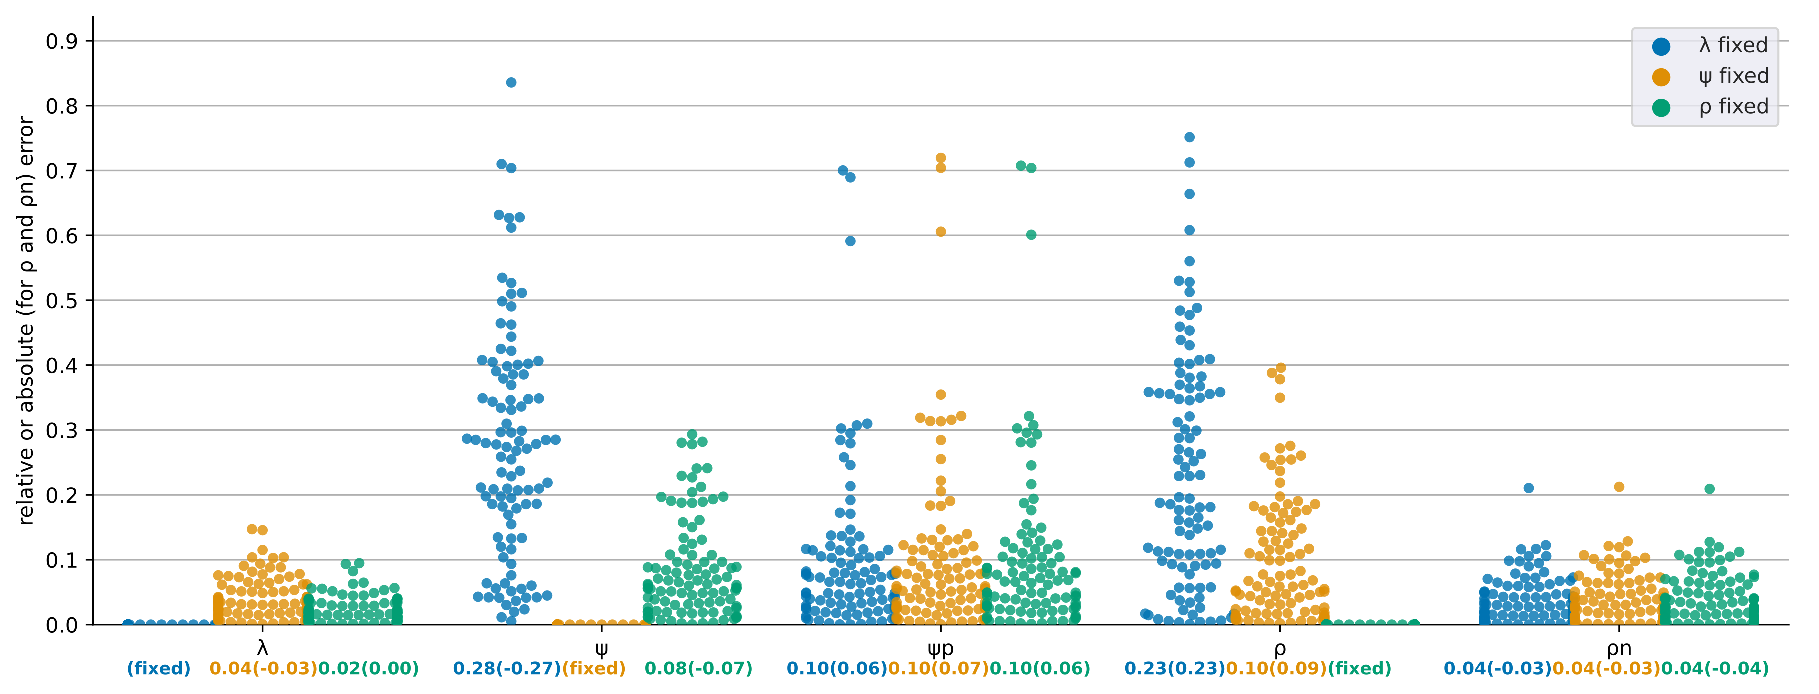
\includegraphics[width=1\textwidth]{Fig_errors.eps}
\caption{Comparison of inference accuracy of bdpn on a data set of 100 trees of 500--1\,000 tips each, with either $\lambda$ (blue), $\psi$ (orange) or $\rho$ (green) parameter being fixed to its real value.
We show the swarmplots (coloured by fixed parameter) of relative errors for each test tree and parameter, which are measured as the normalized distance between the estimate and the real value. Average relative error (and in parentheses average bias, calculated on normalized values) are displayed for each parameter and method below their swarmplot. For $\rho$ absolute values are shown instead of normalized ones. } 
\label{fig:sim} 
\end{figure}
 
 \begin{table}[!h]\centering
\small
\caption{Percentage of simulated trees for which the real parameter values were withing the estimated 95\% CIs. \smallskip}
\begin{tabular}{c|ccc}
\textbf{parameter} & \textbf{$\lambda$ fixed} & \textbf{$\psi$ fixed} & \textbf{$\rho$ fixed} \\
\toprule 
 $\lambda$ & -- &  82\% & 92\% \\
 $\psi$ & 34\% & -- & 78\% \\
 $\rho$ & 20\% & 51\%  & -- \\
 $\psi_p$ & 95\% & 94\% & 95\% \\
 $\rho_n$ & 69\% & 67\% & 64\% \\
\bottomrule
\end{tabular}
\label{tbl:ci}
\end{table}


\subsection{Application: HIV-B epidemic in the UK}
We applied our estimator to asses the partner notification in HIV-infected patients in the UK. We used the dated phylogenetic tree from our recent study of HIV drug resistance in the UK~\citep{zhukovaModelingDrugResistance2023}. The tree represents the UK HIV-B epidemic between 1960s and 2016, its tips represent viruses sampled from 39\,130 individuals between 1996 and 2016. The samples used for the tree reconstruction were obtained from the UK HIV Drug resistance database~\citep{Dunn2007}.

Between 2012 and 2015, in the UK antiretroviral treatment (ART) of HIV-infected individuals  was initiated when their CD4 count dropped below 350 cells/mL~\citep{williamsBritishHIVAssociation2012}. However ``if a patient with a CD4 cell count > 350 cells/mL wishes to start ART to reduce the risk of transmission to partners, this decision is respected and ART is started''~\citep{williamsBritishHIVAssociation2012}. Before 2012, treatment started with an even lower CD4 (i.e. later). The British HIV Association 2015 guidelines recommend all individuals with suspected or diagnosed primary HIV infection ``are offered immediate ART''~\citep{churchillBritishHIVAssociation2016}. To have a more homogeneous setting in terms of access to ART, awareness of the HIV infection, etc., we cut the dated tree between 2012 and 2015, and estimated the BD-PN parameters on the 2012--2015 forests. 

According to the \href{https://webarchive.nationalarchives.gov.uk/ukgwa/20181112132123mp_/https://assets.publishing.service.gov.uk/government/uploads/system/uploads/attachment_data/file/602942/HIV_in_the_UK_report.pdf}{``Towards elimination of HIV transmission, AIDS and HIV-related deaths in the UK''}
 report, the estimated total number of people living with HIV in the UK in 2015 was 101\,200 (97\,500 to 105\,700). % in 2012 this number was 98\,400 (93\,500-104\,300) [\href{HIV in the United Kingdom: 2013 Report}{https://webarchive.nationalarchives.gov.uk/ukgwa/20181112133715mp_/https://assets.publishing.service.gov.uk/government/uploads/system/uploads/attachment_data/file/326601/HIV_annual_report_2013.pdf}]. Moreover these document report about 400 HIV-related deaths per year. 
According to our estimate~\citep{zhukovaModelingDrugResistance2023}, 66.5\% of the HIV-infected individuals in the UK were infected with HIV-B. We hence estimated that in 2015 67\,298 (64\,837, 70\,291) people were living with HIV-B. Our tree contains 39\,047 tips sampled by the end of 2015. Hence, it accounts for about 58\% (56\%, 60\%) of the total number of individuals living with HIV-B in the UK. However this estimate does not take into account deaths of the HIV-infected individuals over the years, which would increase the total number of HIV-infected individuals by 2015, and decrease the proportion of individuals represented by our tree. We therefore tested several sampling probabilities $\rho=$0.6; 0.5; 0.4.
 
 
Using $\rho=0.6$, we estimated the following parameter values: $\lambda=0.262$, $\psi=0.186$, $\psi_p=186.921$, $\rho_n=0.033$, which corresponds to $R_e = 1.4$, infectious time $\frac{1}{\psi} = 5.4$ years, and about 2 days between partner notification and their sampling. The results for $\rho=0.4$ and for $\rho=0.6$ were similar: $R_e$ of respectively $1.5$ and 
$1.3$, infectious time of $5.1$ and $5.6$ years, partner notification probability of $0.033$ in both cases and about 2 days between partner notification and their sampling.
 
The average time of HIV progression to AIDs in the absence of treatment is 10 years, which could serve as an estimate of the infectious time. However, in the UK, 95\% of infected population is on antiretroviral treatment, which, when taken properly, prevents transmission. Hence, the average infectious time represents the average time before starting treatment. Our estimate is approximately 5 years. 


\bibliographystyle{plainnat}
\bibliography{refs}


\end{document}
